\section*{记号约定}

\subsection*{术语与表达式记号}

“自由”一词可能具有两个意思:一个表示\emph{自由理论},即系统的场论哈密顿量中只有场算符的二次型,一个表示\emph{自由电子},即能量就是$\vb*{k}^2/2m$的电子。
前者包括后者但是不完全就是后者,因为能带电子、紧束缚模型等也属于前者。

本文提到的费米子主要是电子,使用一个三维坐标$\vb*{r}$(或者三位动量$\vb*{p}$),以及只有向上和向下两种选择的自旋就可以描述一个电子。
单电子自旋算符为
\begin{equation}
    {\vb*{S}} = \sum_{\alpha, \beta} \ket{\alpha} \vb*{\sigma}_{\alpha \beta} \bra{\beta},
\end{equation}
其中$\alpha$和$\beta$取遍$\uparrow$和$\downarrow$,$\sigma$为泡利矩阵。
在不涉及自旋-轨道耦合的场合,在书写哈密顿量时我们直接略去自旋的下标,这是合理的,因为只需要把不考虑自旋的哈密顿量中的各个产生湮灭算符根据自旋守恒的性质机械地加上自旋下标再求和就能够得到完整的哈密顿量。
在需要实际计算粒子数时就不能这么做了;需要计算总能量时当然也不能这么做。

由于本文不涉及相对论性过程,设$\vb*{a}$为一个矢量,则使用$a$表示其模长。

对离散格点系统,使用$\pair{i, j}$表示最接近的一对格点。(只求和一次,即认为$\pair{i, j}$和$\pair{j, i}$相同)

我们用$\{\alpha | \vb*{a} \}$表示三维欧几里得群$E$的成员,它定义为
\begin{equation}
    \{\alpha | \vb*{a} \} \vb*{r} = \alpha \vb*{r} + \vb*{a},
\end{equation}
其乘法为
\begin{equation}
    \{\alpha_i | \vb*{a}_i \} \{\alpha_j | \vb*{a}_j \} = \{ \alpha_i \alpha_j | \alpha_i \vb*{a}_j + \vb*{a}_i \},
\end{equation}
从而
\begin{equation}
    \{\alpha_i | \vb*{a}_i \}^{-1} = \{ \alpha_i^{-1} | - \alpha_i^{-1} \vb*{a}_i \}.
\end{equation}

\subsection*{单位制}

本文取普朗克单位制,认为$\hbar=c=1$,且$4\pi\epsilon_0=1$,$k_\text{B}=1$。
将本文的计算结果恢复到国际单位制需要遵循以下规则:
\begin{itemize}
    \item 将本文中的$T$替换为$k_\text{B} T$;
    \item 
\end{itemize}
TODO:需要注意“比率”(如热容、态密度等)的定义式中的$T, \dd[3]{\vb*{k}}$等不需要替换。比较好的做法是这样的

$\text{h.c.}$表示厄米共轭,$\text{c.c.}$表示复共轭。

若无特殊说明,$f(z)$定义为近独立费米子的分布函数,即
\[
    f(z) = \frac{1}{\ee^{\beta z} + 1}.
\]

\subsection*{正负号和归一化}

松原格林函数为
\begin{equation}
    G_{AB}(\tau) = - \timeorder \expval*{A(\tau) B(0)}, \quad G_{AB}(\ii \omega_n) = \int_0^\beta \dd{\tau} \ee^{\ii \omega_n \tau} G_{AB}(\tau),
\end{equation}
从频域切换回虚时间的方法是
\begin{equation}
    G_{AB}(\tau) = \frac{1}{\beta} \sum_{\omega_n} G_{AB}(\ii \omega_n) \ee^{- \ii \omega_n \tau}.
\end{equation}
对自由理论,有
\begin{equation}
    G^{0}(\ii \omega_n) = - \int_0^\beta \dd{\tau} \ee^{\ii \omega_n \tau} \timeorder \expval*{c(\tau) c^\dagger(0)} = \frac{1}{\ii \omega_n - \epsilon}.
\end{equation}
做费曼图计算时应当注意传播子是$-G^{0}_{AB}(\ii \omega_n)$。
从松原格林函数延拓到实时间推迟格林函数的方法是将$\ii \omega_n$替换成$\omega + \ii 0^+$。

做自能计算时我们有
\[
    \frac{1}{\begin{gathered}
        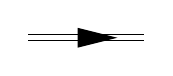
\begin{tikzpicture}[x=0.75pt,y=0.75pt,yscale=-1,xscale=1]
            %uncomment if require: \path (0,300); %set diagram left start at 0, and has height of 300
            
            %Straight Lines [id:da1745692111058319] 
            \draw    (186.35,103.5) -- (235.71,103.5)(186.35,106.5) -- (235.71,106.5) ;
            %Straight Lines [id:da12764386282624862] 
            \draw    (179.71,103.5) -- (214.71,103.5)(179.71,106.5) -- (214.71,106.5) ;
            \draw [shift={(222.71,105)}, rotate = 180] [fill={rgb, 255:red, 0; green, 0; blue, 0 }  ][line width=0.08]  [draw opacity=0] (19.2,-4.8) -- (0,0) -- (19.2,4.8) -- cycle    ;
            \end{tikzpicture}            
    \end{gathered}} = 
    \frac{1}{\begin{gathered}
        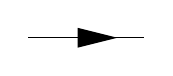
\begin{tikzpicture}[x=0.75pt,y=0.75pt,yscale=-1,xscale=1]
            %uncomment if require: \path (0,300); %set diagram left start at 0, and has height of 300
            
            %Straight Lines [id:da1745692111058319] 
            \draw    (186.35,105) -- (235.71,105) ;
            %Straight Lines [id:da12764386282624862] 
            \draw    (179.71,105) -- (220.71,105) ;
            \draw [shift={(222.71,105)}, rotate = 180] [fill={rgb, 255:red, 0; green, 0; blue, 0 }  ][line width=0.08]  [draw opacity=0] (19.2,-4.8) -- (0,0) -- (19.2,4.8) -- cycle    ;
            \end{tikzpicture}
    \end{gathered}} - \begin{gathered}
        
\begin{tikzpicture}[x=0.75pt,y=0.75pt,yscale=-1,xscale=1]
            %uncomment if require: \path (0,300); %set diagram left start at 0, and has height of 300
            
            %Shape: Circle [id:dp8588117224452179] 
            \draw   (100,144) .. controls (100,130.19) and (111.19,119) .. (125,119) .. controls (138.81,119) and (150,130.19) .. (150,144) .. controls (150,157.81) and (138.81,169) .. (125,169) .. controls (111.19,169) and (100,157.81) .. (100,144) -- cycle ;
            
            % Text Node
            \draw (125,144) node   [align=left] {1PI};
            \end{tikzpicture}
    \end{gathered},
\]
即
\[
    \frac{1}{G} = \frac{1}{G^0} + \begin{gathered}
        
\begin{tikzpicture}[x=0.75pt,y=0.75pt,yscale=-1,xscale=1]
            %uncomment if require: \path (0,300); %set diagram left start at 0, and has height of 300
            
            %Shape: Circle [id:dp8588117224452179] 
            \draw   (100,144) .. controls (100,130.19) and (111.19,119) .. (125,119) .. controls (138.81,119) and (150,130.19) .. (150,144) .. controls (150,157.81) and (138.81,169) .. (125,169) .. controls (111.19,169) and (100,157.81) .. (100,144) -- cycle ;
            
            % Text Node
            \draw (125,144) node   [align=left] {1PI};
            \end{tikzpicture}
    \end{gathered},
\]
或者说
\begin{equation}
    \frac{1}{G} = \frac{1}{G^0} - \Sigma, \quad 
    -\Sigma = \begin{gathered}
        
\begin{tikzpicture}[x=0.75pt,y=0.75pt,yscale=-1,xscale=1]
            %uncomment if require: \path (0,300); %set diagram left start at 0, and has height of 300
            
            %Shape: Circle [id:dp8588117224452179] 
            \draw   (100,144) .. controls (100,130.19) and (111.19,119) .. (125,119) .. controls (138.81,119) and (150,130.19) .. (150,144) .. controls (150,157.81) and (138.81,169) .. (125,169) .. controls (111.19,169) and (100,157.81) .. (100,144) -- cycle ;
            
            % Text Node
            \draw (125,144) node   [align=left] {1PI};
            \end{tikzpicture}
    \end{gathered},
\end{equation}
即单电子(或者别的什么粒子)带相互作用的格林函数的极点展示的能量相比自由格林函数要减去1PI图或者说加上$\Sigma$,这就是所谓自能修正。

\subsection*{主要的字母符号}

费米子的产生湮灭算符为${c}^\dagger$和${c}$,而如果是关于位置的产生湮灭算符,则为${\psi}^\dagger$和${\psi}$。
